%%%%%%%%%%%%%%%%%%%%%%%%%%%%%%%%%%%%%%%%%%%%%%%%%%%%%%%%%%%%%%%%%%%%%%%%%%%%%%%%%%
%%%%%%%%%%%%%%%%%%%%%%%%%%%%%%%%%%%%%%%%%%%%%%%%%%%%%%%%%%%%%%%%%%%%%%%%%%%%%%%%%%
\section{Results} \label{sec_res}
%%%%%%%%%%%%%%%%%%%%%%%%%%%%%%%%%%%%%%%%%%%%%%%%%%%%%%%%%%%%%%%%%%%%%%%%%%%%%%%%%%
%%%%%%%%%%%%%%%%%%%%%%%%%%%%%%%%%%%%%%%%%%%%%%%%%%%%%%%%%%%%%%%%%%%%%%%%%%%%%%%%%%

In this section, we present two Fourier analyses: one where the $S_n$ order is
varied and one where the cell aspect ratio is varied and compare different
methods to solve MIP: Conjugate Gradient (CG), Conjugate Gradient
Preconditioned with Symmetric Gauss-Seidel (PCG-SGS), Conjugate Gradient
Preconditioned with ML using Uncoupled aggregation (PCG-MLU),
Conjugate Gradient Preconditioned with ML using MIS aggregation (PCG-MLMIS),
and AGMG. The computations are performed using a $S_n$ code.

%%%%%%%%%%%%%%%%%%%%%%%%%%%%%%%%%%%%%%%%%%%%%%%%%%%%%%%%%%%%%%%%%%%%%%%%%%%%%%%%%%
\subsection{Fourier Analyses}
%%%%%%%%%%%%%%%%%%%%%%%%%%%%%%%%%%%%%%%%%%%%%%%%%%%%%%%%%%%%%%%%%%%%%%%%%%%%%%%%%%

Assessing some of the properties of Source Iteration accelerated with DSA is
often performed thanks to a Fourier analysis \cite{larsen_dsa,consistent_p1},
where the error is decomposed into different modes. By inspecting the 
damping of the different error modes, the effectiveness of a SI+DSA scheme can 
be studied, often in an infinite homogeneous problem. The largest damping
factor is the spectral radius of the method. The smaller the spectral radius,
the faster the scheme converges. If the spectral
radius is greater than one, the method is unstable. 
\subsubsection{Spectral radius as a function of the $S_n$ order}
This Fourier analysis was carried on a square cell, using a
Gauss-Legendre-Chebyshev (GLC) quadrature. The medium is homogeneous with a 
scattering ratio $c=0.9999$; periodic boundary conditions are used. The results 
are plotted on \Cref{fig_fa_sn}, where the $x-$axis is the mesh size in mean free 
paths and the $y-$axis is the spectral radius. There are four curves corresponding 
to different $S_n$ orders: $S_2$, $S_4$, $S_8$ and $S_{16}$.
\begin{figure}[H]
  \centering
  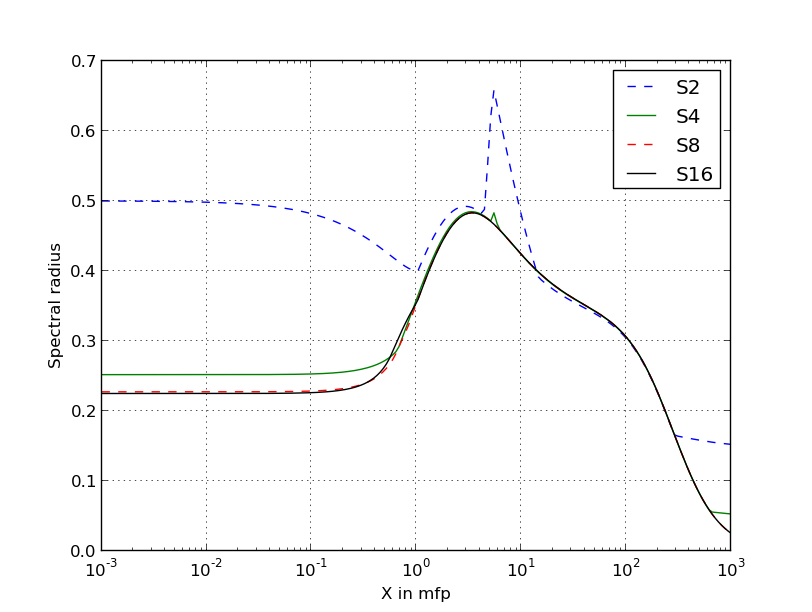
\includegraphics[width=0.5\textwidth]{sn_order_9999}
  \caption{Fourier analysis as a function of the mesh optical thickness
    various}
  \label{fig_fa_sn}
\end{figure}
Looking at \Cref{fig_fa_sn}, we can conclude that MIP is stable for every 
cell size. The spectral radius is always less than 0.5, except for $S_2$ where 
it is about 0.7.
\subsubsection{Spectral radius as a function of the cell aspect ratio}
For this Fourier analysis, we use a $S_{16}$ GLC quadrature. The medium is
again homogeneous with $c=0.9999$ and periodic boundary conditions. 
On \Cref{fig_fa_ar}, the five curves correspond to the following cell aspect 
ratio: $\frac{Y}{X}=\frac{1}{16}$, $\frac{Y}{X}=\frac{1}{4}$,
$\frac{Y}{X}=1$, $\frac{Y}{X}=4$, $\frac{Y}{X}=16$, and $\frac{Y}{X}=100$.
\begin{figure}[H]
  \centering
  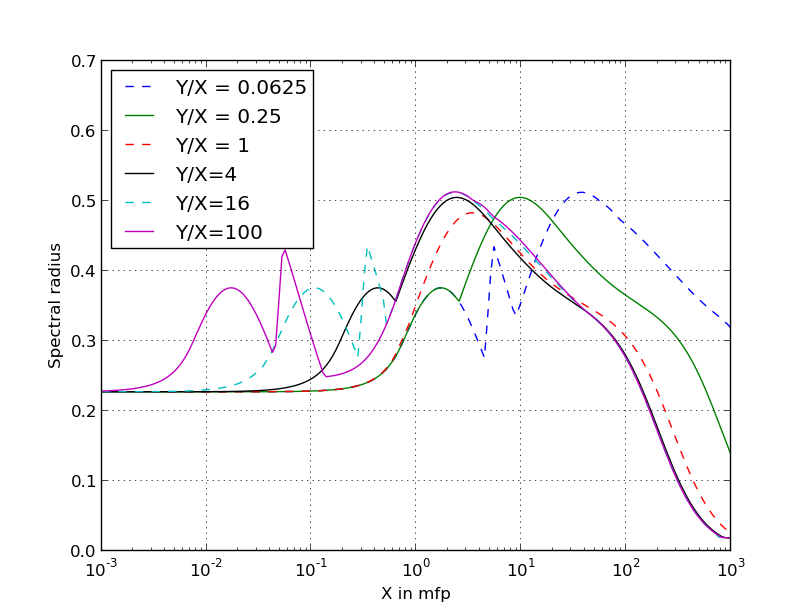
\includegraphics[width=0.5\textwidth]{aspect_ratio_9999_2}
  \caption{Fourier analysis as a function of the mesh optical thickness,
  $S_{16}$, various aspect ratios}
  \label{fig_fa_ar}
\end{figure}
MIP is stable for every aspect ratio, including 100, and the maximum spectral radius
is about 0.5.

%%%%%%%%%%%%%%%%%%%%%%%%%%%%%%%%%%%%%%%%%%%%%%%%%%%%%%%%%%%%%%%%%%%%%%%%%%%%%%%%%%
\subsection{Numerical results using MIP-DSA implemented in an $S_n$ code}
%%%%%%%%%%%%%%%%%%%%%%%%%%%%%%%%%%%%%%%%%%%%%%%%%%%%%%%%%%%%%%%%%%%%%%%%%%%%%%%%%%

\subsubsection{Homogeneous medium test case}  \label{sec_homog}
%%%%%%%%%%%%%%%%%%%%%%%%%%%%%%%%%%%%%%%%%%%%%%%%%%%%%%%%%%%%%%%%%%%%%%%%%%%%%%%%%%

We compare different solvers for MIP-DSA on a homogeneous medium, $100cm
\times 100cm$, $\Sigma_t = 1cm^{-1}$ and $\Sigma_s = 0.999cm^{-1}$, with
vacuum boundary conditions and a source of intensity $1cm^{-3}s^{-1}$. We
use a $S_8$ Gauss-Legendre-Chebyshev quadrature, a Source Iteration solver
with relative tolerance of $10^{-8}$ and a relative tolerance of
$10^{-10}$ for MIP-DSA. The medium is discretized using two different meshes:
\begin{description}
  \item[Quadrilateral grid:] the mesh is composed of 49236 quadrilateral
    cells that to 197052 degrees of freedom.
  \item[Polygonal grid:] the mesh is composed of 45204 triangles, 823
    quadrilaterals, 4978 pentagons, 4155 hexagons, 725 heptagons, and 24
    octagons, for a total of 55909 cells and 193991 degrees of freedom. This
    example will allow us to test MIP and the different preconditioners on a
    mesh composed of different cell types.
\end{description}
The meshes and the solutions of these problems are given on \Cref{homog_test}.
\begin{figure}[H]
  \centering
  \begin{subfigure}{0.45\textwidth}
    \centering
    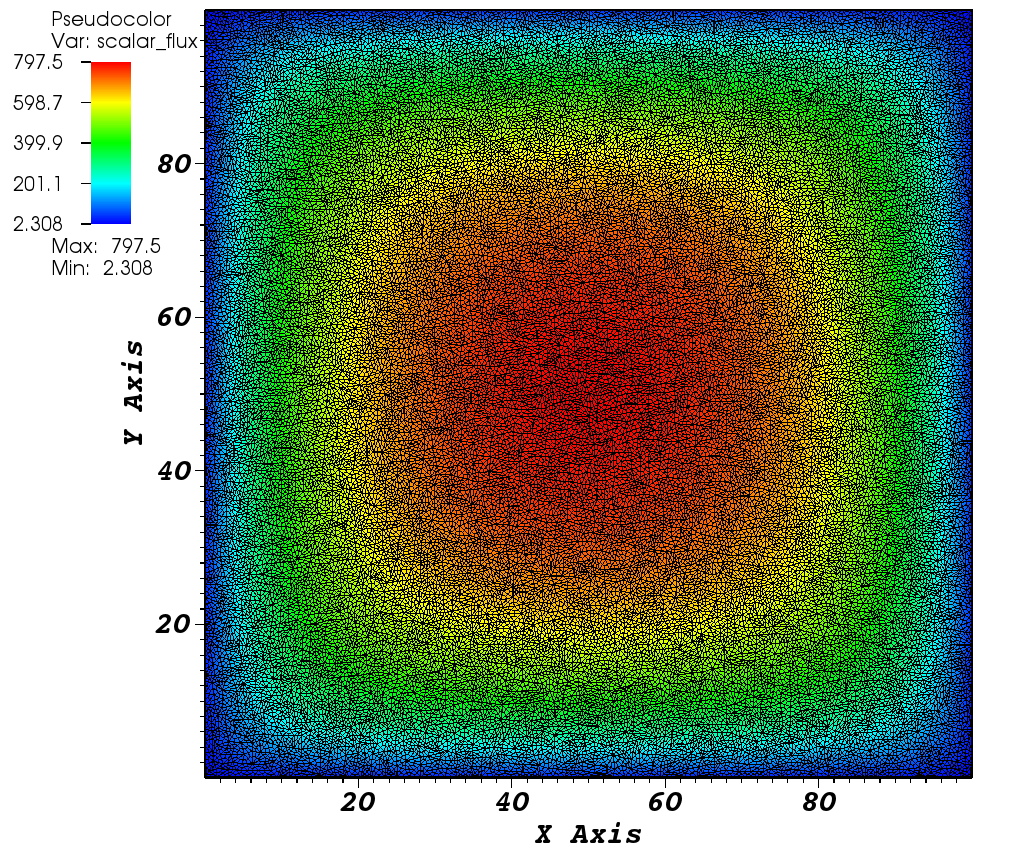
\includegraphics[width=\textwidth]{big_homog_quad_crop}
    \caption{Quadrilateral cells}
  \end{subfigure}
  \begin{subfigure}{0.45\textwidth}
    \centering
    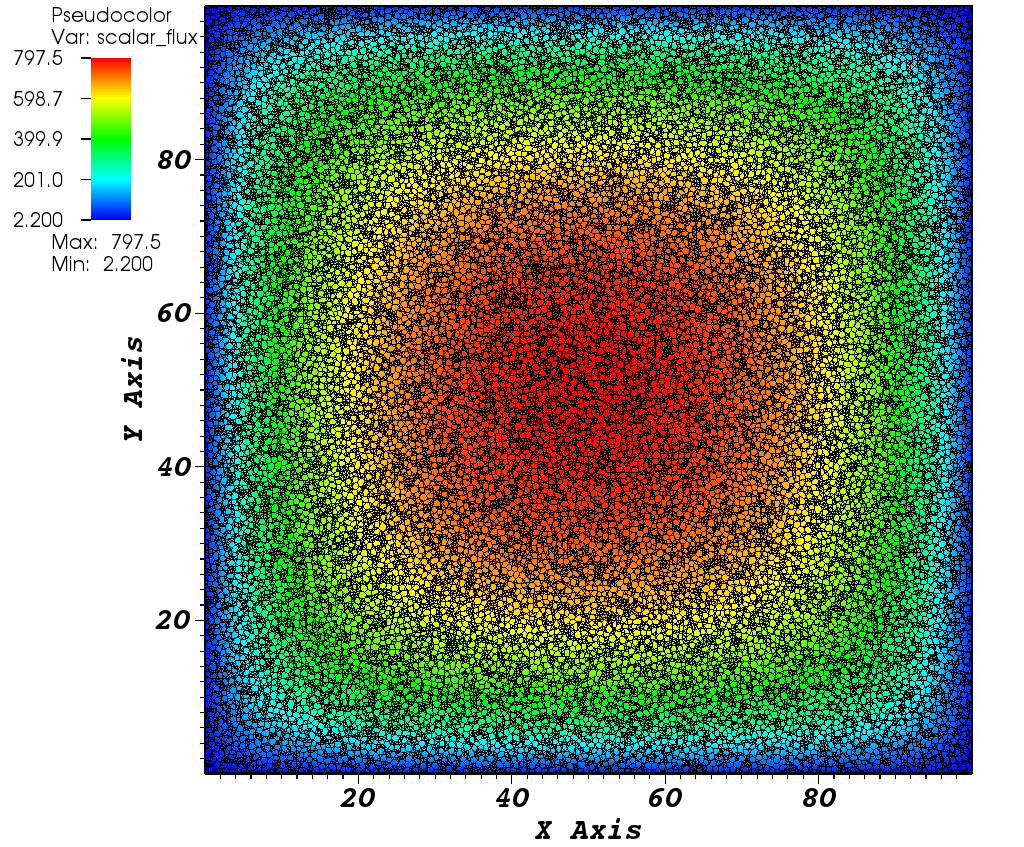
\includegraphics[width=\textwidth]{big_homog_poly_crop}
    \caption{Polygonal cells}
  \end{subfigure}
  \caption{Meshes and scalar fluxes}
  \label{homog_test}
\end{figure}
In \Cref{comparison_homog_quad}, the different solvers, used with the
quadrilateral grid, are compared:
\begin{table}[H]
  \begin{center}
    \caption{Comparison of different preconditioners for quadrilateral cells}
    \begin{tabular}{|c|c|c|c|c|c|c|}
      \hline
      & No-DSA & CG & PCG-SGS & PCG-MLU & PCG-MLMIS & AGMG \\
      \hline
      SI iterations   & 7311    & 24      & 24       & 24      & 24      & 24 \\
   Precond init (s)   & NA      & NA      & 0.171358 & 1.8255  & 9.56078 & 0.332 \\
MIP calculation (s)   & NA      & 1095.7  & 1311.76  & 192.622 & 197.632 & 29.9727 \\
      CG iterations   & NA      & 56649   & 17332    & 630     & 604     & 578 \\
Total calculation (s) & 39176.7 & 1264.98 & 1477.95  & 363.202 & 367.841 &
      194.568 \\
      \hline
    \end{tabular}
    \label{comparison_homog_quad}
  \end{center}
\end{table}
In \Cref{comparison_homog_quad}, SI iterations is the number iteration of 
Source Iteration needed to solve the problem, Precond init is the time, in
seconds, needed to initialize the preconditioner used by CG, MIP calculation
is the total time, in seconds, spent solving DSA during the calculation, CG
iterations is the total number of CG iterations used to solve MIP, and Total
calculation is the time, in seconds, needed to solve the problem. We can see
than PGC-ML and AGMG require about the same number of iterations (two orders
of magnitude less than for CG). However, AMG is much faster than PCG-ML. This 
is because each PCG-SGS iteration is much slower than one
unpreconditioned CG iterations. Profiling of the code reveals that the
bottleneck is the function 
\emph{Ifpack\_PointRelaxation::ApplyInverseSGS\_FastCrsMatrix} of Trilinos. This
function applies the forward and the backward substitutions required by SGS.
It is unclear why these substitutions are so costly. We can see in
\Cref{comparison_homog_quad}, the reason why there is such a big
difference between AGMG and PCG-ML is due to SGS. SGS is used as pre- and
post-smoother in ML and the function
\emph{Ifpack\_PointRelaxation::ApplyInverseSGS\_FastCrsMatrix} is once again the
bottleneck of the method.

The different solvers, used with the polygonal grids, are compared in
\Cref{comparison_homog_poly}:
\begin{table}[H]
  \begin{center}
    \caption{Comparison of different preconditioners for polygonal cells}
    \begin{tabular}{|c|c|c|c|c|c|c|}
      \hline
      & No-DSA & CG & PCG-SGS & PCG-MLU & PCG-MLMIS & AGMG \\
      \hline
      SI iterations   & 7311    & 23      & 23      & 23      & 23      & 23 \\
   Precond init (s)   & NA      & NA      & 0.06388 & 1.73379 & 8.0426  & 0.388 \\
MIP calculation (s)   & NA      & 877.861 & 1263.31 & 198.63  & 191.989 &
      31.242 \\
      CG iterations   & NA      & 46262   & 16712   & 652     & 603     & 555 \\
Total calculation (s) & 42666.7 & 1060.53 & 1447.53 & 382.275 & 384.422 &
      216.946 \\
      \hline
    \end{tabular}
    \label{comparison_homog_poly}
  \end{center}
\end{table}
We see that using different types of cells in the same mesh does not affect
the performance of MIP-DSA or that of its preconditioners.

\subsubsection{Heterogeneous medium}
%%%%%%%%%%%%%%%%%%%%%%%%%%%%%%%%%%%%%%%%%%%%%%%%%%%%%%%%%%%%%%%%%%%%%%%%%%%%%%%%%%

In this example, a heterogeneous geometry with three materials is used. It is 
composed of 184 triangles, 3720 quadrilaterals and 2791 regular hexagons of 
side $0.05cm$ for a total of 6695 cells and 32178 degrees of freedom (spatial 
unknowns per angular direction). The domain is $5.28275cm$ by $4.6cm$. 
Reflective boundary conditions are used. A $S_{16}$ Gauss-Legendre-Chebyshev 
quadrature is used. The SI solver has a relative tolerance of 
$10^{-8}$ and the relative tolerance for MIP is $10^{-10}$. \Cref{hex_zones}
shows the problem geometry and the material properties are in given
\Cref{hex_prop}.
\begin{figure}[H]
  \centering
  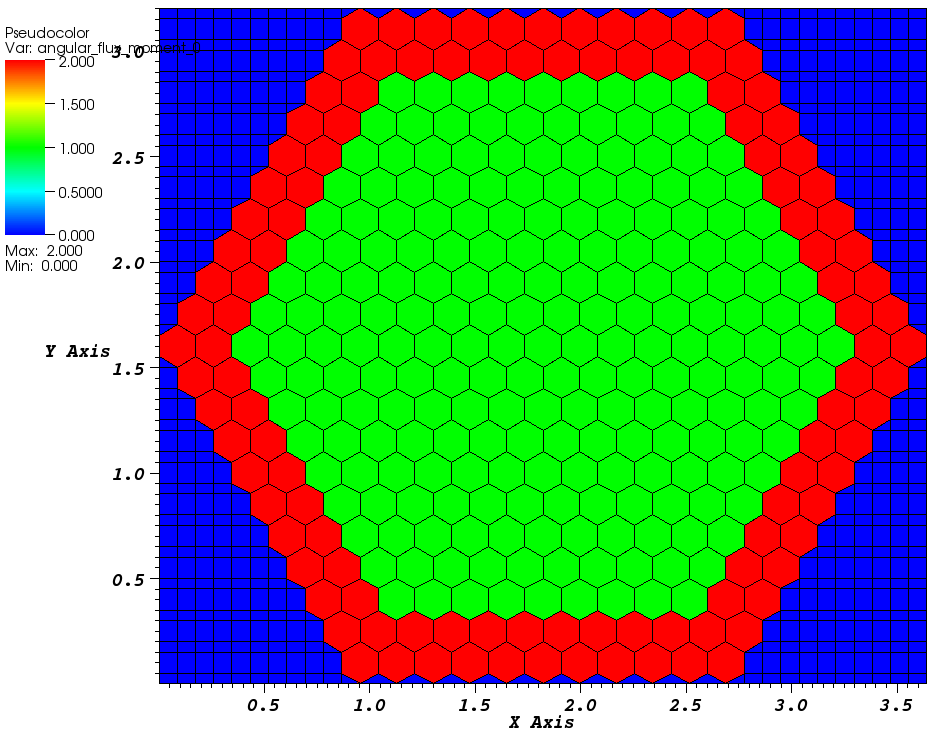
\includegraphics[width=0.4\textwidth]{source_crop}
  \caption{Zones of the heterogeneous test domain}
  \label{hex_zones}
\end{figure}
\begin{table}[H]
  \begin{center}
    \caption{Properties of the different zones}
    \begin{tabular}{|c|c|c|c|}
      \hline
       & Inner zone & Intermediate zone & Outer zone \\
      $\Sigma_t$ $(cm^{-1})$ & 1.5 & 1.0 & 1.0 \\
      $\Sigma_s$ $(cm^{-1})$ & 1.4999 & 0.999 & 0.3 \\
     source $(cm^{-3}s^{-1}$ & 1.0 & 0.0 & 0.0 \\
      \hline
    \end{tabular}
    \label{hex_prop}
  \end{center}
\end{table}
The different solvers are compared in \Cref{comparison_hex}.
\begin{table}[H]
  \begin{center}
    \caption{Comparison of preconditioners, heterogeneous problem}
    \begin{tabular}{|c|c|c|c|c|c|c|}
      \hline
      & No-DSA & CG & PCG-SGS & PCG-MLU & PCG-MLMIS & AGMG\\
      \hline
      SI iterations & 278     & 17      & 17        & 17       & 17      & 17  \\
   Precond init (s) & NA      & NA      & 0.0160661 & 0.368768 & 1.41632 &
      0.07  \\
MIP calculation (s) & NA      & 58.422  & 126.93    & 33.2225  & 31.3045 &
      2.924 \\
      CG iterations & NA      & 12214   & 6679      & 415      & 386     & 248  \\
Total calculation (s) & 910.566 & 120.889 & 190.413 & 99.7524  & 97.4666 &
      70.6424 \\      
      \hline
    \end{tabular}
    \label{comparison_hex}
  \end{center}
\end{table}
We can see that the remarks of \Cref{sec_homog} made for the homogeneous test
remain the same. MIP-DSA is effective even with heterogeneous medium and AGMG is
still the fastest solver. It is interesting to note that, contrary to the
homogeneous tests where the number of CG iterations remained similar for all
algebraic multigrid preconditioners, in this heterogeneous test AGMG requires
significantly fewer iterations than the Trilinos implementation, PCG-MLU, 
and PCG-MLMIS.

\subsubsection{AMR mesh}
%%%%%%%%%%%%%%%%%%%%%%%%%%%%%%%%%%%%%%%%%%%%%%%%%%%%%%%%%%%%%%%%%%%%%%%%%%%%%%%%%%

In this example \cite{mip}, the domain is $10cm\times 10cm$. The left and bottom
boundaries are reflective whereas the right and the top boundaries are vacuum. 
There are 10720 cells: 10482 quadrilaterals, 236 pentagons,
and 2 hexagons for a total of 43120 degrees of freedom. 
As in the previous example, the domain is composed if three zones (see
\Cref{zone_amr} and \Cref{prop_amr}).
\begin{figure}[H]
  \centering
  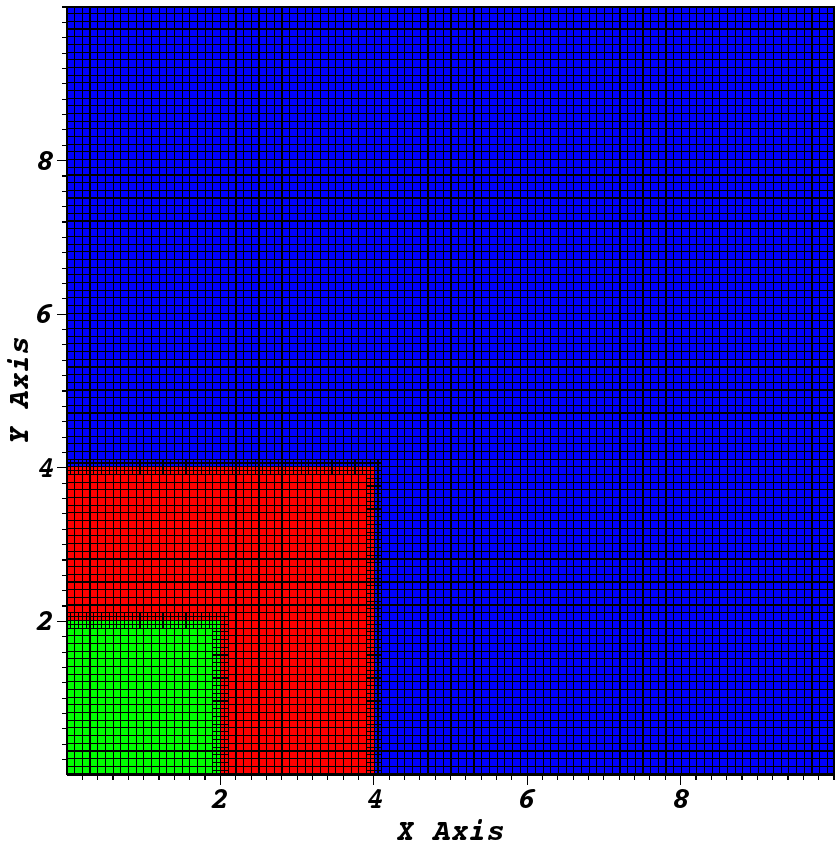
\includegraphics[width=6cm]{zone_amr}
  \caption{Zones of the AMR test domain}
  \label{zone_amr}
\end{figure}
\begin{table}
  \begin{center}
    \caption{Properties}
    \begin{tabular}{|c|c|c|c|}
      \hline
      & Green zone & Red zone & Blue zone \\
    $\Sigma_t$ $(cm^{-1})$ & 1.5 & 1. \\
    $\Sigma_s$ $(cm^{-1})$ & 1.44 & 0.9 & 0.3 \\
  Source $(cm^{-3}s^{-1})$ & 1.0 & 0.0 & 0.0 \\
      \hline
    \end{tabular}
    \label{prop_amr}
  \end{center}
\end{table}
The distribution of cells is given \Cref{fig_pol_dist}.
\begin{figure}[H]
  \centering
  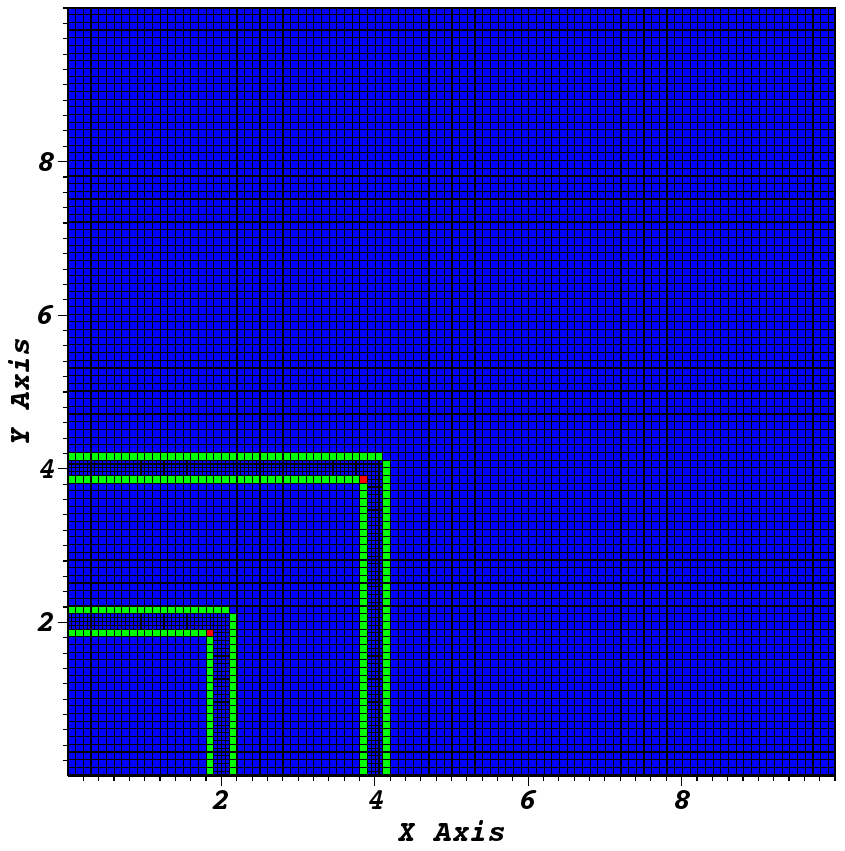
\includegraphics[width=6cm]{polygon_amr}
  \caption{Polygons distribution}
  \label{fig_pol_dist}
\end{figure}
where the blue cells are quadrilaterals, the green cells are pentagons, and
the red cells are hexagons. This mesh is typical of a mesh obtained after one 
level of adaptive mesh
refinement (the cells at the interface of different materials have been refined
once). We see that instead of introducing hanging nodes, we have introduce
pentagons and hexagons in the mesh.
A $S_{16}$ GLC quadrature is employed. The tolerance on SI is $10^{-8}$ and
the tolerance on the CG solvers is $10^{-10}$.
The different solvers are compared in \Cref{table_amr}.
\begin{table}[H]
  \caption{Comparison of preconditioners on AMR mesh}
  \begin{center}
    \begin{tabular}{|c|c|c|c|c|c|c|}
      \hline
       & No-DSA & CG & PCG-SGS & PCG-MLU & PCG-MLMIS & AGMG \\
      \hline
   SI iterations & 184     & 19      & 19       & 19      & 19       & 19 \\
Precond init (s) & NA      & NA      & 0.043463 & 0.358002 & 1.19301 & 0.0111\\
MIP calculation (s) & NA   & 48.1908 & 81.0992  & 25.2699 & 25.0699  & 
      2.56198\\
   CG iterations & NA      & 11300   & 4734     & 361     & 361      & 264 \\
     Total calculation (s) & 802.985 & 138.825 & 172.423  & 116.018 & 116.517  &
      94.1963\\
      \hline
    \end{tabular}
    \label{table_amr}
  \end{center}
\end{table}
The conclusions are similar to the ones made for our previous tests.

\subsubsection{Rectangular cells}
%%%%%%%%%%%%%%%%%%%%%%%%%%%%%%%%%%%%%%%%%%%%%%%%%%%%%%%%%%%%%%%%%%%%%%%%%%%%%%%%%%

\red{When the aspect ratio is high and the scattering ratio is close to one, MIP
becomes ill-conditioned.} In the next two examples, the domain is square $100cm
\times 100cm$ with vacuum boundaries. There are 10000 cells and thus, 40000
degrees of freedom. The relative tolerance on SI is $10^{-8}$ and the relative
tolerance for CG is $10^{-10}$. We use a $S_8$ GLC quadrature, $\Sigma_t =
1cm^{-1}$, and $\Sigma_s = 0.999cm^{-1}$. The source is $1n/(cm^3s)$. In the
first test, the domain is discretized by 100 cells along $x$ and 100 cells
along $y$, i.e., square cells with aspect ratio of one. In the second run, 
the domain is discretized by 1000 cells along $x$ and 10 cells along $y$ 
(the aspect ratio is 100).
\begin{table}[H]
  \caption{Comparison of preconditioners on rectangular grid with an aspect
  ratio of 1}
  \begin{center}
    \begin{tabular}{|c|c|c|c|c|c|c|}
      \hline
       & No-DSA & CG & PCG-SGS & PCG-MLU & PCG-MLMIS & AGMG \\
      \hline
      SI iterations & 7311      & 21      & 21      & 21       & 21      & 21 \\
   Precond init (s) & NA        & NA      & 0.01422 & 0.051373 & 1.13144 &
      0.044 \\
MIP calculation (s) & NA        & 32.3825 & 73.8422 & 24.0707  & 25.0065 &
      1.7114 \\
      CG iterations & NA        & 8363    & 4853    & 376      & 375     &
      221\\
Total calculation (s) & 7356.96 & 56.8993 & 98.2609 & 50.1247  & 51.5396 &
      25.9306 \\
      \hline
    \end{tabular}
    \label{table_ar_1}
  \end{center}
\end{table}
\begin{table}[H]
  \caption{Comparison of preconditioners on rectangular grid with an aspect
  ratio of 100}
  \begin{center}
    \begin{tabular}{|c|c|c|c|c|c|c|}
      \hline
       & No-DSA & CG & PCG-SGS & PCG-MLU & PCG-MLMIS & AGMG \\
      \hline
      SI iterations & 7304    & 24      & 24        & 24       & 24      & 24 \\
   Precond init (s) & NA      & NA      & 0.0164239 & 0.362463 & 1.03128 & 0.052 \\
MIP calculation (s) & NA      & 372.227 & 742.902   & 941.06   & 922.258 &
      6.93176 \\
      CG iterations & NA      & 84802   & 43466     & 14180    & 13896   & 821 \\
Total calculation (s) & 9035.6 & 414.301 & 784.77   & 985.796  & 966.77  &
      44.7032 \\
      \hline
    \end{tabular}
    \label{table_ar_100}
  \end{center}
\end{table}                  
As expected, solving the MIP-DSA equations requires more CG iterations when the aspect
ratio increases. PCG-MLU and PCG-MLMIS are significantly more affected by the
increase in the aspect ratio than the other methods. AGMG is the least
affected by the change of aspect ratio and is the best performing
preconditioner.
